\documentclass{beamer}
\usepackage{dirtytalk}
\usetheme{metropolis}
\usepackage{hyperref}
\usepackage{tikz}
\institute{Georgia Tech}
\usepackage[utf8]{inputenc}

\title{MATH 4802: Presentation 4}
\author{Anna, Haoyun, Jim, Kevin,
Pavan, Sean, Sergei, Walter, Zachary Brumbach, Jiaying Deng}
\date{\today}

\begin{document}

\begin{frame}
\titlepage
\end{frame}

\section{Introduction}
\begin{frame}{Problem Statement}
\begin{quote}
    A round-robin tournament of $2n$ teams lasted for $2n-1$ days, as follows. On each day, every team played one game against another team, with one team winning and one team losing in each of the $n$ games. Over the course of the tournament, each team played every other team exactly once. Can one necessarily choose one winning team from each day without choosing any team more than once?
\end{quote}
\end{frame}

\section{Representing as a Graph Problem}
\begin{frame}{Bipartite Representation}
We chose to represent this problem as a bipartite graph, with partition $L$ being the set of teams, and partition $R$ being the set of days. An edge $(l, r)$ exists in the graph $G$ if team $l$ wins on day $r$.
In the example shown below, team $l_1$ won on all 3 days, $l_2$ won on $r_1$ and $r_2$, $l_3$ won on $r_3$, and $l_4$ never won.
    \begin{center}
        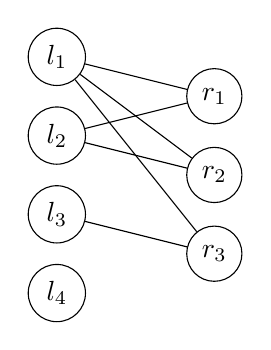
\begin{tikzpicture}
            \node[shape=circle, draw=black] (a) at (-1, 0){$l_1$};
            \node[shape=circle, draw=black] (b) at (-1, -1){$l_2$};
            \node[shape=circle, draw=black] (c) at (-1, -2){$l_3$};
            \node[shape=circle, draw=black] (d) at (-1, -3){$l_4$};
            
            \node[shape=circle, draw=black] (e) at (1, -0.5){$r_1$};
            \node[shape=circle, draw=black] (f) at (1, -1.5){$r_2$};
            \node[shape=circle, draw=black] (g) at (1, -2.5){$r_3$};
            
            \path [-] (a) edge node[left] {} (e);
            \path [-] (a) edge node[left] {} (f);
            \path [-] (a) edge node[left] {} (g);
            
            \path [-] (b) edge node[left] {} (e);
            \path [-] (b) edge node[left] {} (f);
            
            \path [-] (c) edge node[left] {} (g);
        \end{tikzpicture}
    \end{center}
\end{frame}

\begin{frame}{Reduction to Matching}
By representing our problem with a bipartite graph, we have reduced our problem to asking whether or not there is a matching\footnote{A set of edges with no common vertices} covering $R$.

On a bipartite graph, this is solvable via \textit{Hall's Marriage Theorem}, which states that there is a matching covering $R$ if and only if $\forall S \subseteq R, |E_{L, S}| \geq |S|$, where $|E_{L, S}|$ is the set of edges between $L$ and $S$. Thus, to determine if we can choose a unique winning team for each day, we need to prove or disprove the above inequality.
\end{frame}

\section{Leveraging Hall's Marriage Theorem}
\begin{frame}{Proving the Inequality}
Let $S$ be a subset of $R$. Then, define the set of teams that have won at least one game on any day in S, $W(S)$ as:
\begin{equation}
    W(S) = \{l \in L: \exists r \in S, (l, r) \in G\}
\end{equation}
We note that since there is at least one edge per team that won a game:
\begin{equation}
    |E_{L, S}| \geq |W(S)|
\end{equation}
As such, to prove the inequality for Hall's Marriage Theorem, it suffices to prove 
\begin{equation}
\forall S \subseteq R, |W(S)| \geq |S|
\end{equation}
We will do so via proof by contradiction.
\end{frame}

\begin{frame}{Proof by Contradiction}
We start by assuming $|W(S)| < |S|$. Let $t$ be a team that loses their game each day in $|S|$. Since:
\begin{equation}
   |W(S)| < |S| \leq |R| = 2n-1 < |L| = 2n 
\end{equation}
$t$ must exist, as there are more teams than there are teams with at least one win.

However, since each team plays a different team each day, this means that $t$ must have lost to $|S|$ unique teams, implying that $|W(S)| \geq |S|$. This is a contradiction, in turn proving that:
\begin{equation}
\forall S \in R, |W(S)| \geq |S|
\end{equation}
\end{frame}

\begin{frame}{Finishing the Proof}
By results (3) and (5), we have satisfied the condition for Hall's Marriage Theorem, so there must exist a matching that covers $R$. Since a matching consists of edges with unique vertices, this means that each day in $R$ has a unique corresponding team in $L$.

Thus, there is a way to pick a unique winning team for each day.
\end{frame}

\end{document}
